\documentclass{scrartcl}  % scrartcl of scrreprt
\usepackage{SIunits}
% Include all project wide packages here.
\usepackage{fullpage}
\usepackage{polyglossia}
\setmainlanguage{dutch}
\usepackage{csquotes}
\usepackage{graphicx}
\usepackage{epstopdf}
\usepackage{pdfpages}
\usepackage{caption}
\usepackage[list=true]{subcaption}
\usepackage{float}
%\usepackage{mathtools}
\usepackage{standalone}
\usepackage{import}
\usepackage{tocloft}
\usepackage{wrapfig}
\usepackage{authblk}
\usepackage{array}
\usepackage{booktabs}
\usepackage[toc,page,title,titletoc]{appendix}
\usepackage{xunicode}
\usepackage{amsmath}
\usepackage{fontspec}
\usepackage{unicode-math}
\usepackage[
    backend=bibtexu,
	texencoding=utf8,
bibencoding=utf8,
    style=ieee,
    sortlocale=nl_NL,
    language=auto
]{biblatex}
\usepackage{listings}
\newcommand{\includecode}[3][c]{\lstinputlisting[caption=#2, escapechar=, style=#1]{#3}}
\newcommand{\superscript}[1]{\ensuremath{^{\textrm{#1}}}}
\newcommand{\subscript}[1]{\ensuremath{_{\textrm{#1}}}}


\newcommand{\chapternumber}{\thechapter}
\renewcommand{\appendixname}{Bijlage}
\renewcommand{\appendixtocname}{Bijlagen}
\renewcommand{\appendixpagename}{Bijlagen}

\usepackage[hidelinks]{hyperref} %<--------ALTIJD ALS LAATSTE
  
\renewcommand{\familydefault}{\sfdefault}

\setmainfont[Ligatures=TeX]{Myriad Pro}
\setmathfont{Asana Math}
\setmonofont{Lucida Console}

\usepackage{titlesec, blindtext, color}
\definecolor{gray75}{gray}{0.75}
\newcommand{\hsp}{\hspace{20pt}}
\titleformat{\chapter}[hang]{\Huge\bfseries}{\chapternumber\hsp\textcolor{gray75}{|}\hsp}{0pt}{\Huge\bfseries}
\renewcommand{\familydefault}{\sfdefault}
\renewcommand{\arraystretch}{1.2}
\setlength\parindent{0pt}

%For code listings
\definecolor{black}{rgb}{0,0,0}
\definecolor{browntags}{rgb}{0.65,0.1,0.1}
\definecolor{bluestrings}{rgb}{0,0,1}
\definecolor{graycomments}{rgb}{0.4,0.4,0.4}
\definecolor{redkeywords}{rgb}{1,0,0}
\definecolor{bluekeywords}{rgb}{0.13,0.13,0.8}
\definecolor{greencomments}{rgb}{0,0.5,0}
\definecolor{redstrings}{rgb}{0.9,0,0}
\definecolor{purpleidentifiers}{rgb}{0.01,0,0.01}


\lstdefinestyle{csharp}{
language=[Sharp]C,
showspaces=false,
showtabs=false,
breaklines=true,
showstringspaces=false,
breakatwhitespace=true,
escapeinside={(*@}{@*)},
columns=fullflexible,
commentstyle=\color{greencomments},
keywordstyle=\color{bluekeywords}\bfseries,
stringstyle=\color{redstrings},
identifierstyle=\color{purpleidentifiers},
basicstyle=\ttfamily\small}

\lstdefinestyle{c}{
language=C,
showspaces=false,
showtabs=false,
breaklines=true,
showstringspaces=false,
breakatwhitespace=true,
escapeinside={(*@}{@*)},
columns=fullflexible,
commentstyle=\color{greencomments},
keywordstyle=\color{bluekeywords}\bfseries,
stringstyle=\color{bluestrings},
identifierstyle=\color{purpleidentifiers}
}

\lstdefinestyle{vhdl}{
language=VHDL,
showspaces=false,
showtabs=false,
breaklines=true,
showstringspaces=false,
breakatwhitespace=true,
escapeinside={(*@}{@*)},
columns=fullflexible,
commentstyle=\color{greencomments},
keywordstyle=\color{bluekeywords}\bfseries,
stringstyle=\color{redstrings},
identifierstyle=\color{purpleidentifiers}
}

\lstdefinestyle{xaml}{
language=XML,
showspaces=false,
showtabs=false,
breaklines=true,
showstringspaces=false,
breakatwhitespace=true,
escapeinside={(*@}{@*)},
columns=fullflexible,
commentstyle=\color{greencomments},
keywordstyle=\color{redkeywords},
stringstyle=\color{bluestrings},
tagstyle=\color{browntags},
morestring=[b]",
  morecomment=[s]{<?}{?>},
  morekeywords={xmlns,version,typex:AsyncRecords,x:Arguments,x:Boolean,x:Byte,x:Char,x:Class,x:ClassAttributes,x:ClassModifier,x:Code,x:ConnectionId,x:Decimal,x:Double,x:FactoryMethod,x:FieldModifier,x:Int16,x:Int32,x:Int64,x:Key,x:Members,x:Name,x:Object,x:Property,x:Shared,x:Single,x:String,x:Subclass,x:SynchronousMode,x:TimeSpan,x:TypeArguments,x:Uid,x:Uri,x:XData,Grid.Column,Grid.ColumnSpan,Click,ClipToBounds,Content,DropDownOpened,FontSize,Foreground,Header,Height,HorizontalAlignment,HorizontalContentAlignment,IsCancel,IsDefault,IsEnabled,IsSelected,Margin,MinHeight,MinWidth,Padding,SnapsToDevicePixels,Target,TextWrapping,Title,VerticalAlignment,VerticalContentAlignment,Width,WindowStartupLocation,Binding,Mode,OneWay,xmlns:x}
}

%defaults
\lstset{
basicstyle=\ttfamily\small,
extendedchars=false,
numbers=left,
numberstyle=\ttfamily\tiny,
stepnumber=1,
tabsize=4,
numbersep=5pt
}
\addbibresource{../../library/bibliography.bib}

\author{ Jorden {Kerkhof}  }
\title{EPO3: Eindrapport - VGA-controller}

\begin{document}

\section{VGA-controller}
\label{ch:vga}
\section{Specificaties}

De VGA-controller is een belangrijk component in ons systeem. Deze zorgt er namelijk voor dat alles wat berekend wordt in de module ook daadwerkelijk zichtbaar gemaakt zal worden. De VGA-controller legt de verbinding tussen de rest van ons systeem en een scherm, hierdoor is fysiek te zien wat er gebeurt in het systeem. 

De specificaties van de VGA-controller zijn uitgedrukt in de in- en uitgangen van dit component. Hieronder een overzichtelijk tabel daarvan. Bij de vectoren is de grootte gegeven in parameters. Deze parameters zijn terug te vinden in de beschrijving van het package file, welke eerder is besproken in dit verslag.

\begin{table}[H]
	\centering
	\caption{Specificaties van de VGA Controller }
	\label{tab:spec-vgacontroller}
	\begin{tabular}{c c c}
		\hline\hline
	 	Naam & Modus & Type\\
	 	\hline	
		clk & in & std\_logic \\ 
		reset\_n & in & std\_logic \\ 
		vgahsync & out & std\_logic \\ 
		vgavsync & out & std\_logic \\ 
		vga\_claim & out & std\_logic \\ 
		ramaddr & out & std\_logic\_vector(SizeRAMAddr-1 downto 0) \\
		vga\_read & out & std\_logic \\
		vga\_can\_access & in & std\_logic \\
		asb & in & std\_logic \\
	  	\hline\hline
	\end{tabular}
\end{table}

\section{Ontwerp en implementatie}

Aan het begin van de entity worden eerst een aantal constanten gecreëerd. Deze zijn afgesteld op de grootte van ons resolutie en hoe snel we het scherm willen verversen. In het ontwerp is al grotendeels besproken welke signalen binnenkomen bij de VGA-controller. De ingangen zijn vrij standaard. De ingangen zijn clk(clock), reset\_n (negative reset), vga\_can\_access en asb( active screen buffer). De uitgangen zijn vgahsync, vgavsync, vga\_claim, ramaddr en vga\_read. Vgahync en vgavsync zijn hier de horizontalen en verticale synchronisatie pulsen. De kleur wordt op het juiste moment direct verbonden van de RAMController naar de VGA-poort. Ramaddr is het adres van de pixel waar het scherm op dit moment is. Vga\_claim is een signaal dat aangeeft dat de vga-controller op dit moment toegang heeft tot de RAM. VGA\_read geeft aan dat de VGA-controller de RAM gegevens uitleest.
\\\\
In de behaviour wordt er als eerste  een aantal belangrijke constanten en signalen gedeclareerd. De periode van de horizontale en de verticale synchronisatie pulsen bepalen hoe lang er doorgeteld moet worden totdat je het hele scherm bent afgegaan. We hebben deze zo ingesteld dat ze iets groter zijn dan onze resolutie daadwerkelijk is. Dit om ervoor te zorgen dat als de vga-controller aan het tekenen is buiten het scherm dat de waarden even weer goed kunnen worden ingelezen. Omdat we een negatieve reset hebben, gaat de code werken als de reset hoog is. Vervolgens begint de vga-controller te synchroniseren. Hij begint buiten het scherm en zorgt ervoor dat de juiste data aan de ingangen staat. Vervolgens begint hij van links naar recht, van boven naar beneden het scherm in te vullen. Elk moment dat hij bij een bepaalde pixel is geeft hij dit adres door aan de RAM-controller. Deze leest uit de RAM welke kleur deze pixel moet hebben en stuurt dit rechtstreeks door naar de vga-controller. Deze stuurt dat vervolgens gelijk door naar de uitgang zodat de correcte kleur op het goede moment en het juiste tijdstip wordt afgebeeld. Omdat onze clock uiteindelijk te langzaam is om goed te kunnen functioneren, hebben we als oplossing om vgavsync aan te passen. Deze wordt vier keer langzamer en we tekenen elke pixel dan ook 4 keer. Dit zorgt er tevens ook voor dat we mooiere pixels hebben. 


\section{VHDL simulatie}
Om te testen of de VHDL-code werkte hebben we een testbench geschreven. Hier laten we de vga\_can\_access hoog worden, zodat de vga-controller in zijn werk zal gaan. Hieronder een overzicht van de resultaten van de simulatie.
\begin{figure}[H]
\centering
		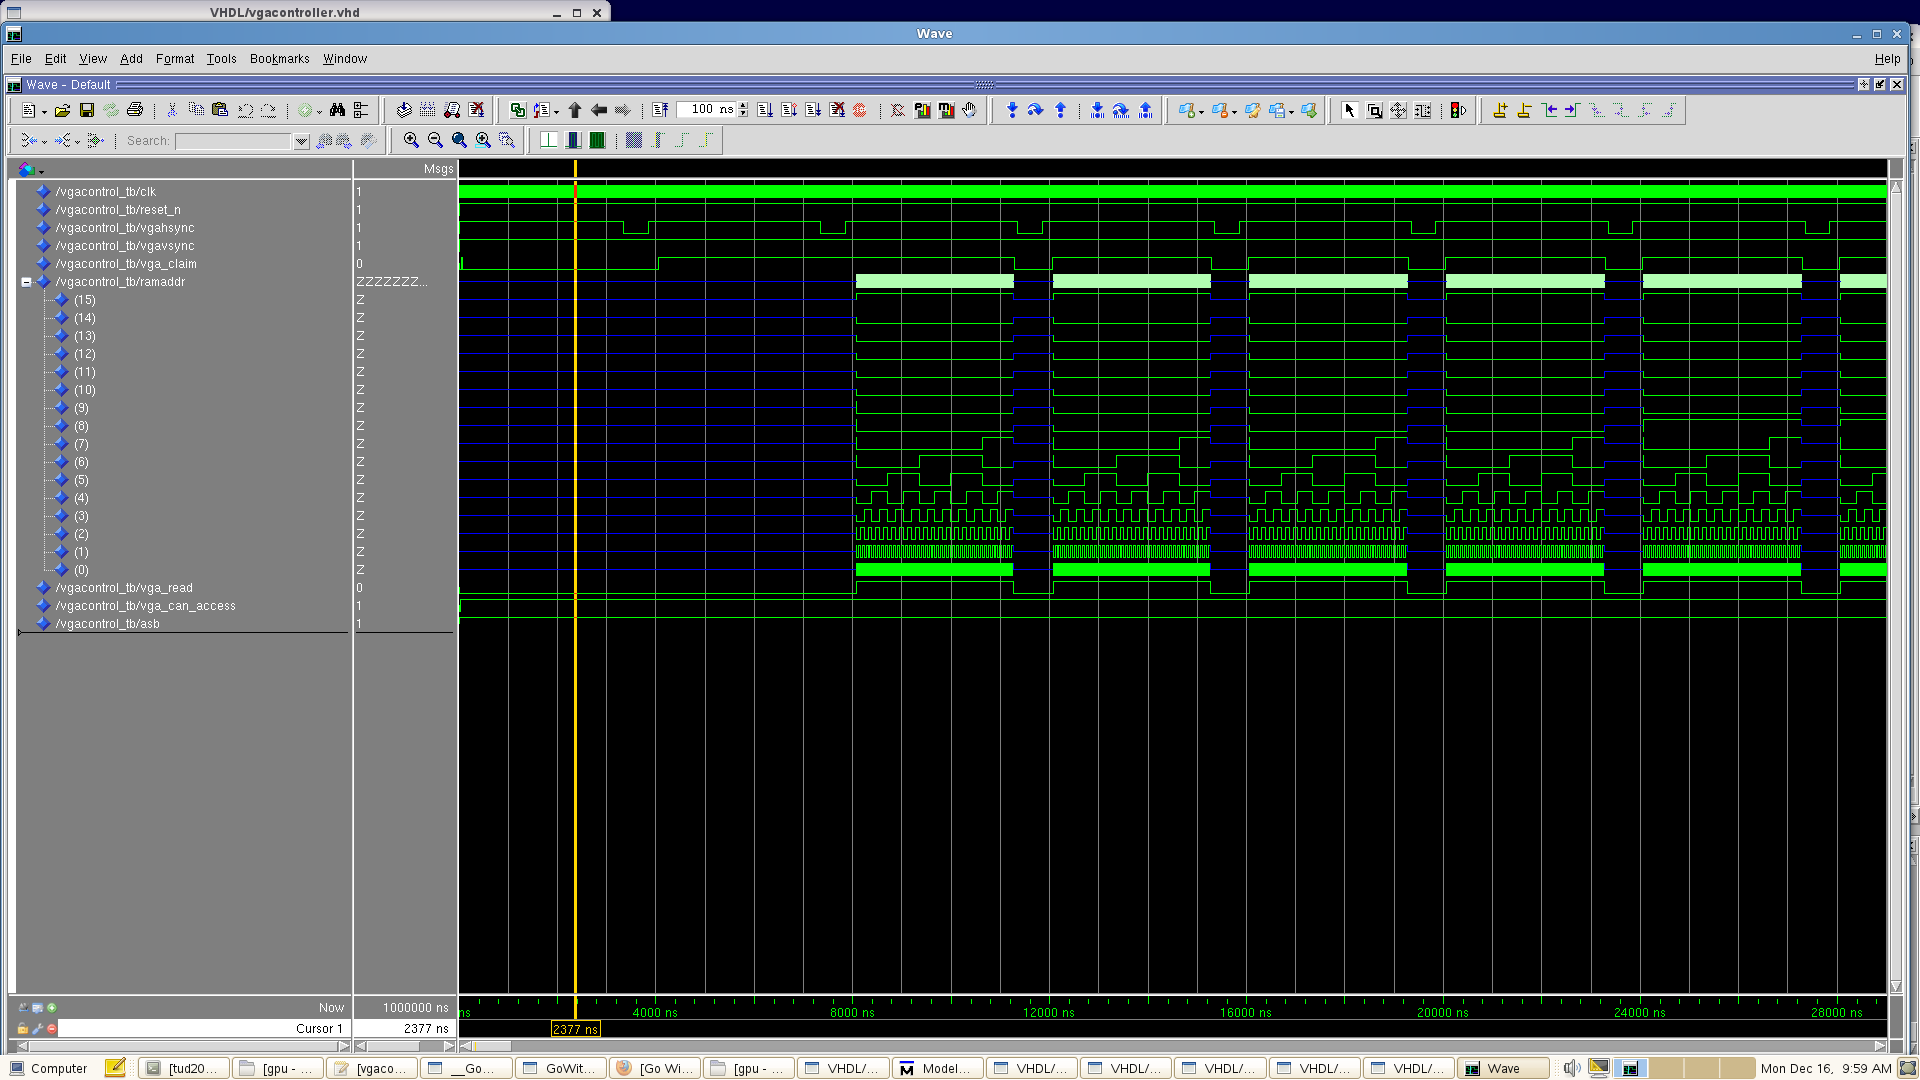
\includegraphics[width=1\textwidth]{resource/simmodvgafinal.png}
		
		\caption{Het resultaat van de simulatie in Modelsim.}
		\label{fig:sim}
\end{figure}
Uit figuur \ref{fig:sim} kunnen we dus afleiden dat de vga-controller telkens een hele regel afgaat, vervolgens even verder gaat om de waarden in te lezen en een volgende regel weer helemaal afgaat. 

\section{Synthese en lay-out}
Voor de synthese hebben we het programma GoWithTheFlow gebruikt. Hier kwam een gesynthetiseerde versie uit, met een bijbehorend design.
\begin{figure}[H]
\centering
		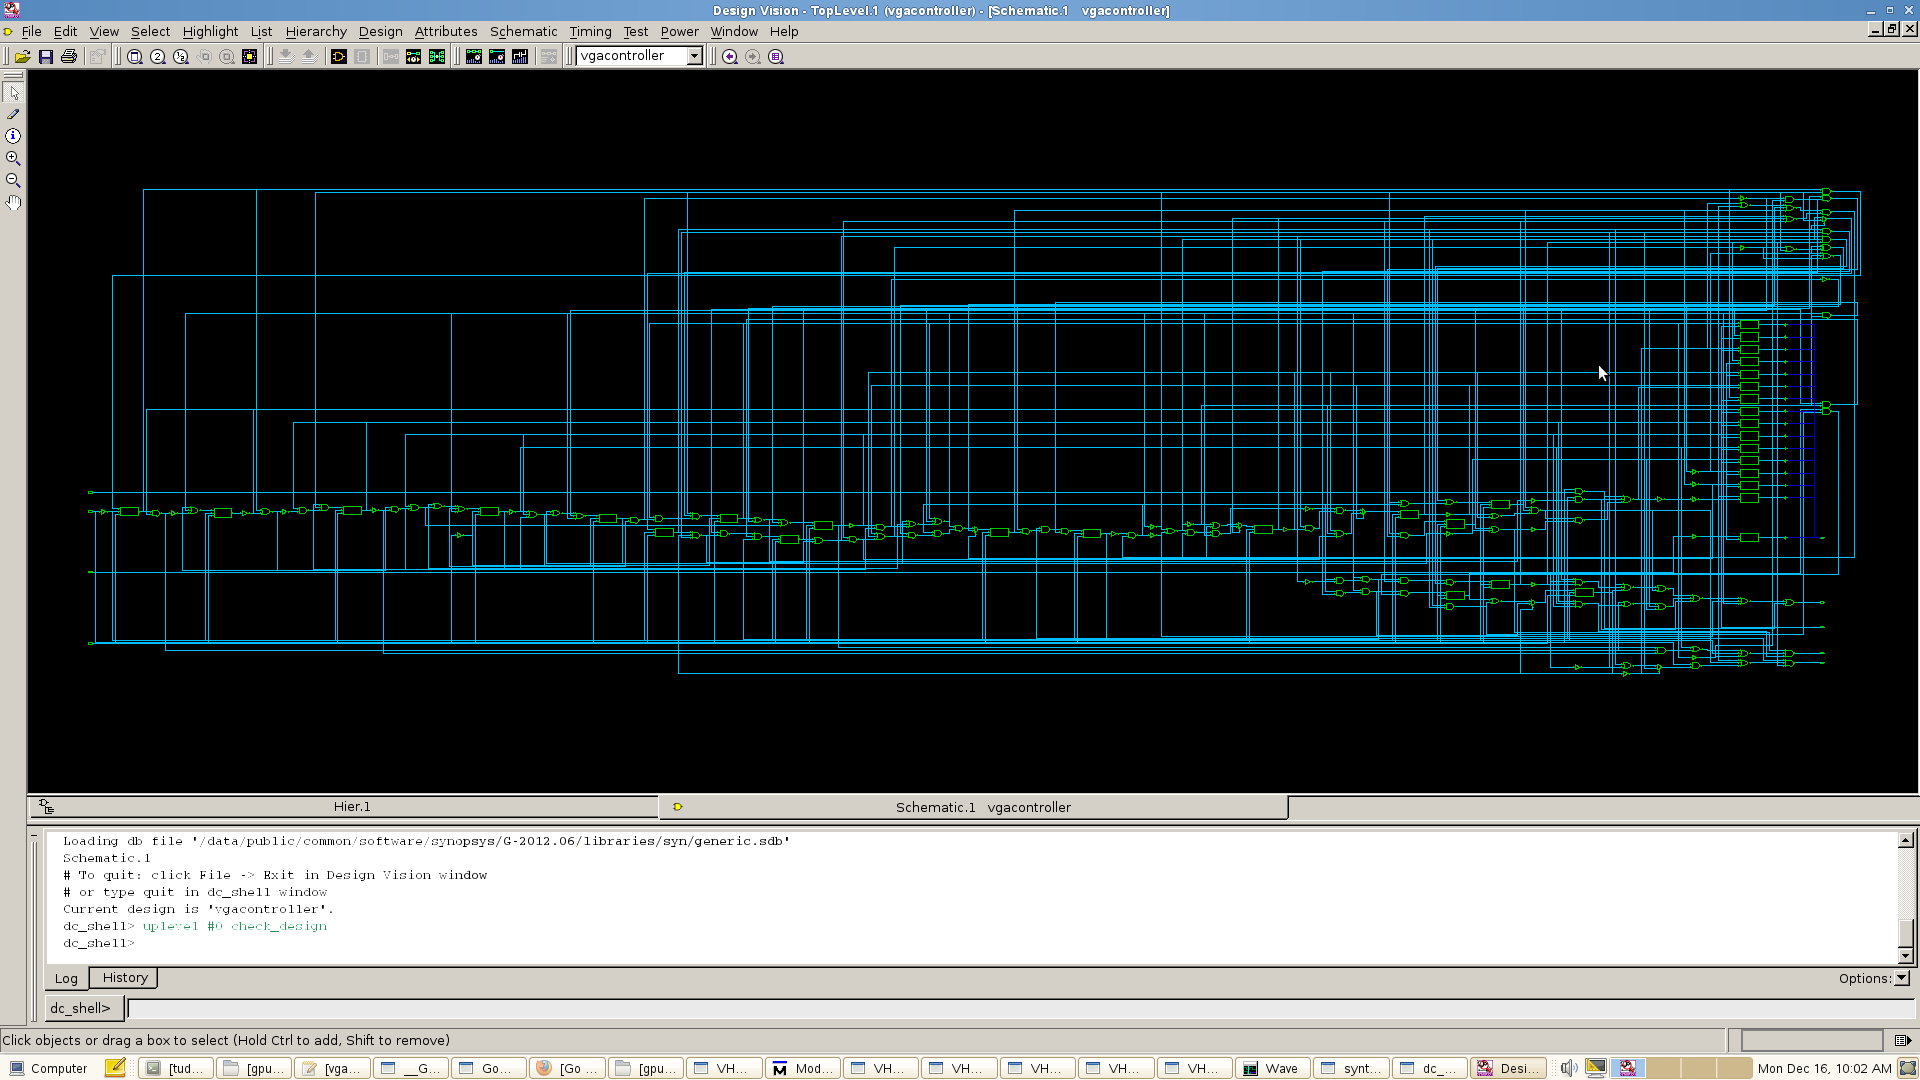
\includegraphics[width=1\textwidth]{resource/circuitvgafinal.png}
		
		\caption{Het resultaat van de synthese van de VGA-Controller}
		\label{fig:circuit}
\end{figure}
Hieruit bleek dat de uiteindelijke efficiëntie voor dit component 41.91\% is. Het liefst heb je natuurlijk een efficientie van 100\%. Helaas is dit ons niet gelukt, omdat wij ook rekening moeten houden met de grootte van het geheel. Aangezien wij een beperkt aantal transistoren tot onze beschikking hebben, hebben we getracht zo weining mogelijk transistoren te gebruiken. Uiteindelijk hebben een totaaloppervlakte van  4152 transistoren, waarvan er 1740 daadwerkelijk worden gebruikt. Dit is te verklaren doordat er in de entity heel wat constanten worden gedefiniëerd, speciaal alleen voor de vga-controller. Dit is lastig te synthetiseren en geeft een lagere effeciëntie van je transistorgebruik.
Bij de extracted versie van de VHDLl controleer je of de code ook nog werkt wanneer je hem hebt geïmplementeerd en omgezet in hardware componenten. Uit onze simulatie hiervan bleek dat de resultaten bijna precies overeen kwamen met de simulatie van de normale testbench. De meest voorkomende fout, was wanneer de uitgang op high-impedance ('Z') werd gezet. Dit kon na de synthese niet goed worden uitgevoerd, en werd danwel een '1' of een '0'. Opzich geeft dit geen problemen omdat VGA\_claim ook op '0' staat. Er zal dus niks gebeuren richting de vga-poort.

\section{Switch-level simulatie}
De gesynthetiseerde code is gesimuleerd met SLS. De resultaten hiervan zijn te vinden in \ref{fig:switch}. 

\begin{figure}[H]
\centering
		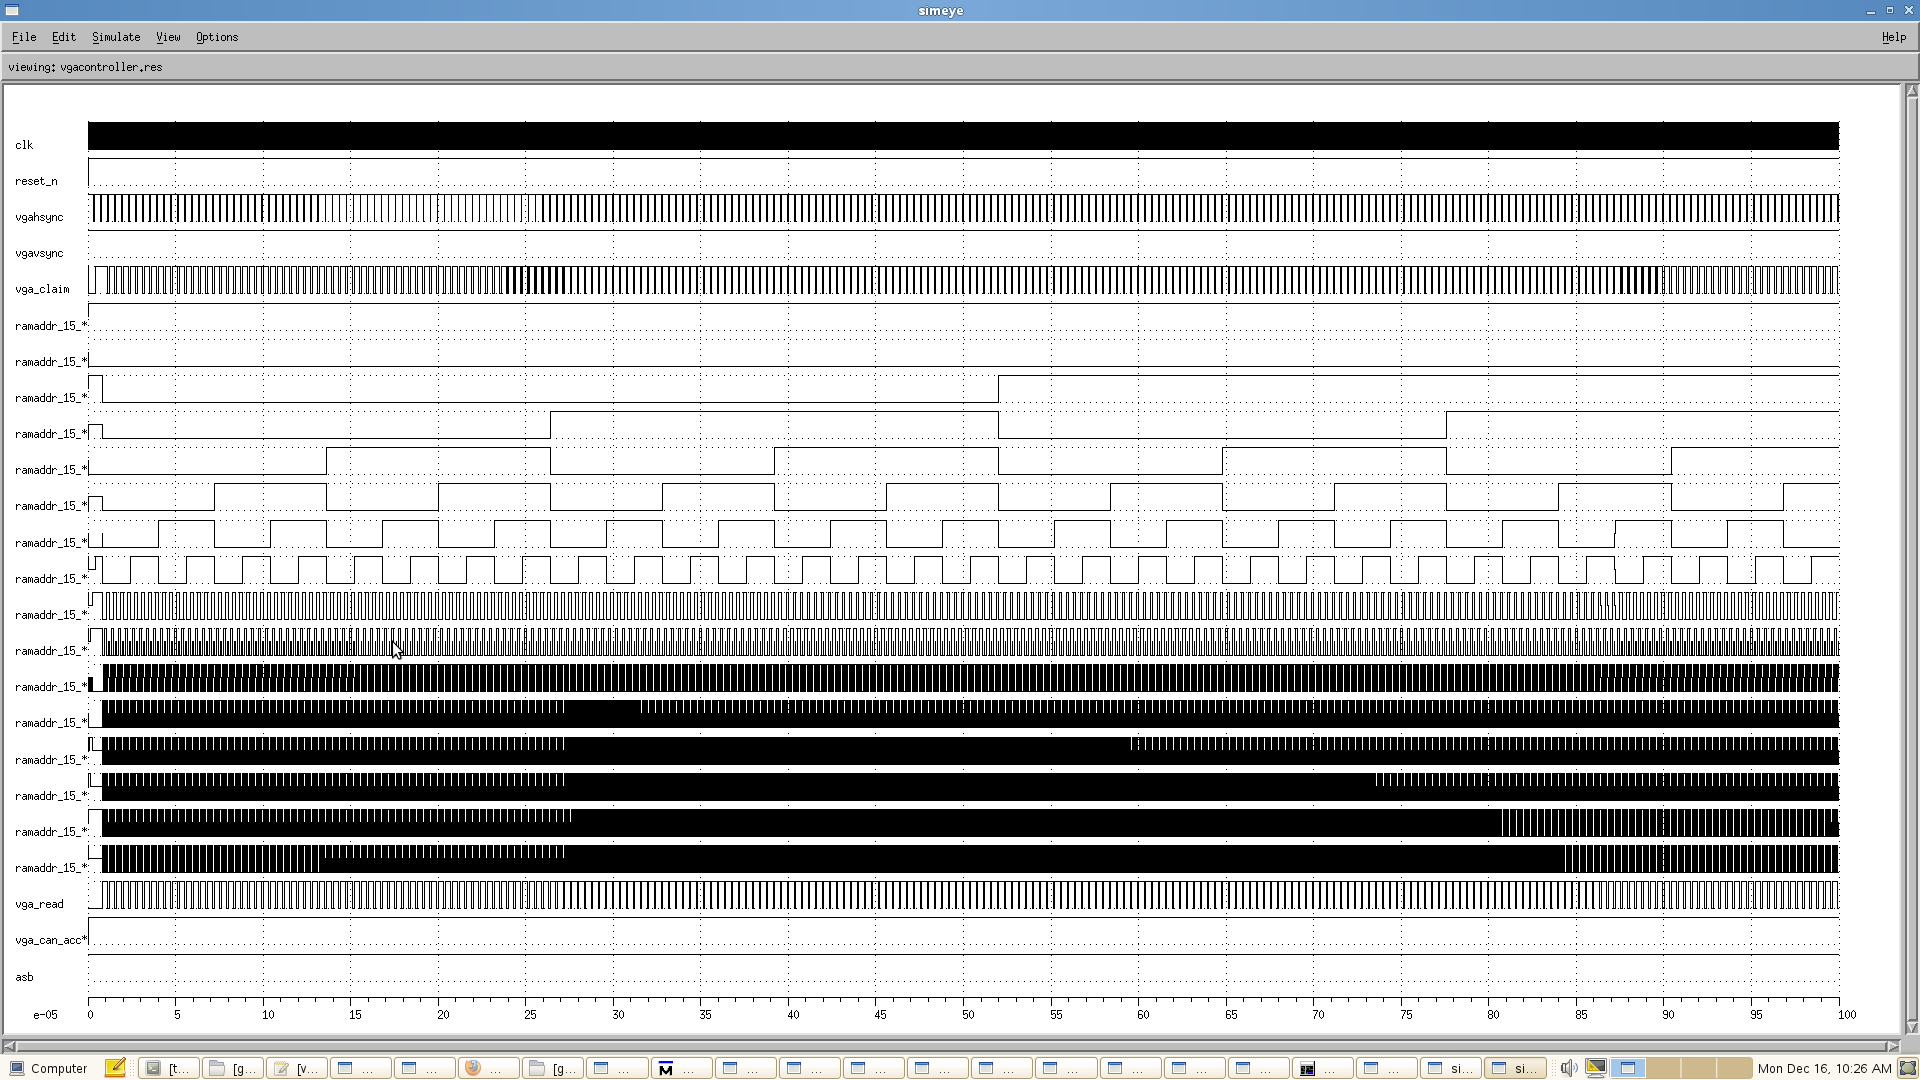
\includegraphics[width=1\textwidth]{resource/simslsvga-final.png}
		
		\caption{De SLS simulatie van de gesynthetiseerde schakeling van VGA-Controller}
		\label{fig:switch}
\end{figure}
Vervolgens zijn deze uitkomsten vergeleken met de resultaten van de originele testbench, welke gesimuleerd is in ModelSim. Hieruit bleek dat beide codes hetzelfde resultaat opleverden en geen errors veroorzaakten. Dit houdt in dat de vga-controller goed synthetiseerbaar is. De hardware zal uiteindelijk geen problemen opleveren en zal dezelfde resultaten moeten afleveren als de simulatie van de testbench zou doen. 


\section{Conclusie}
Uit meerdere simulaties blijkt dat de code werkt. De resultaten van de simulatie komen overeen met de gewenste resultaten. Dit houdt in dat de code naar behoren werkt en goed te implementeren is. De code zal waarschijnlijk geen problemen geven als deze geïmplementeerd wordt.

De VHDL beschrijving en testbench staan in Bijlagen \ref{appsec:vgacontroller.vhd}, \ref{appsec:vgacontroller-behaviour.vhd} en \ref{appsec:vgacontroller-tb.vhd}.


\end{document}

